\documentclass[paper=a4, twoside=false, fontsize=12pt, parskip=half,
                bibliography=totoc, listof=totoc]{scrbook}

% General packages
\usepackage{sourdough}

% Basic attributes
\author{Hendrik Kleinwächter}
\title{The Sourdough Framework}

\begin{document}
\thispagestyle{empty}
\setlength{\unitlength}{1mm}
\noindent\begin{picture}(0,0)(1,-1)
\put(-16.3,-265){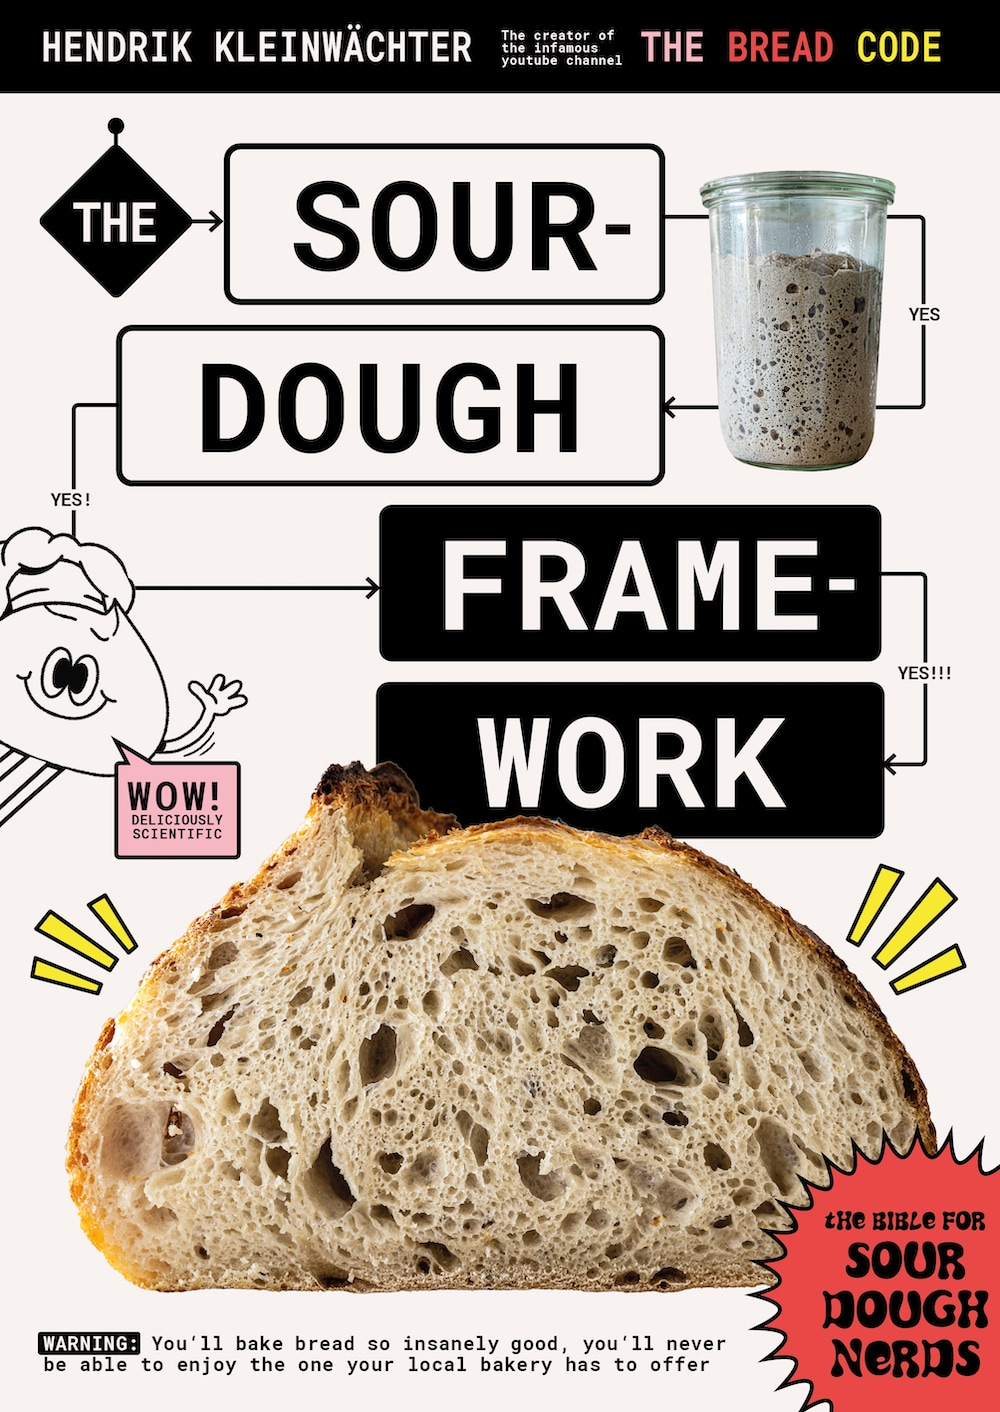
\includegraphics[width=1.33\linewidth]{cover/cover-page.jpg}}
\end{picture}

\newpage
\thispagestyle{empty}

\rule{1pt}{\textheight} % Vertical line
 % Whitespace between the vertical line and title page text
\hspace{0.05\textwidth}
 % Paragraph box for holding the title page text, adjust the width to move the
% title page left or right on the page
%\raggedleft%
\parbox[b]{0.75\textwidth}{%
{\Huge\bfseries The Sourdough Framework}\\[2\baselineskip] % Title
{\large\textit{Version: \today}}\\[4\baselineskip]
{\Large\textsc{Hendrik Kleinwächter}} % Author name, lower case for consistent small caps

% Whitespace between the title block and the copyright text
\vspace{0.5\textheight}

{\noindent The full source code for the book is available at \\
\url{https://github.com/hendricius/the-sourdough-framework/} under CC-BY-SA
license. Do not hesitate to report mistakes or sug\-gestions for
improvements. A hardcover version of the book is also available. More information here:
\url{https://www.breadco.de/hardcover-book}}\\[\baselineskip]
}

\titlepage

{%
\hypersetup{hidelinks}
\ifdefined\HCode\else\tableofcontents\fi
}

If there is one food Germany is known for, it is probably bread.
There are thousands of varieties in Germany,
and making it has been an integral part of our culture.

My bread journey began during childhood. My mother, being a parent
of 3, would always use Saturdays to bake a delicious loaf for the family.
It was a white fluffy sandwich bread, and she made it within one to two hours using store-bought yeast.
Being a bit more experienced, I now realize it's
ideal to wait a little while before cutting into your bread, but back then,
we kids couldn't wait. Mom would cut for us a few slices straight from the oven, and we would
immediately proceed to pour butter or jam on each slice. Within minutes, 1 kg of
flour would be consumed. Bread became an integral part of my weekly food.

I was lucky that my parents could afford a yearly ski trip to
Alto Adige in northern Italy. In the small town called Valdaora, we
would try new restaurants every year, yet always end up in our favorite
pizza place. The pizzas there were incredible. The dough
alone was so tasty that we would order just the bread with a
bit of olive oil and salt.

Of course, my question would always be, ``Mom, can we make this at home, too, please?''
So over the years, we became friends with the owners and would receive
more and more clues as how to make the perfect pizza dough. There
are no secret ingredients inside. It's just flour, water, salt, and a bit of yeast.
How can such a simple combination of ingredients create such an incredibly delicious
pizza dough? My parents, being creatures of habit, would return every year with us,
and every year, my interest would grow. At home, Mom and I attempted to replicate
the recipe. We tried baking on a stone and on a steel. We tried adding oil to the dough and herbs
to the pizza sauce. We fell into an endless cycle of experiments. However, we never managed
to get close to the experience we had while on vacation.

Some years passed, and I eventually began my studies in the small German city of Göttingen.
For the first time, I was faced with shopping for my own bread. It was never
on my mind to actually start baking it for myself. I would just buy 
a good loaf while shopping at the supermarket. My favorite variety
was a Schwarzbrot, Korn an Korn. It’s a very dark and hearty rye bread
with added berries and sunflower seeds. Being a little naïve,
I'd never before examined the packaging of what I was buying. One day, that
changed.

I looked at the label and was shocked. The seemingly
healthy bread consisted of so many other things aside from flour and water.
The black color was not coming from the flour, but from caramelized sugar.
The packaging stated it was a sourdough bread, but then why was there additional yeast?
I thought that if it was really sourdough, it shouldn't require additional yeast, and I
soon realized that something was wrong with the bread I was buying.
I proceeded to check the other supermarket breads, only to discover that they, too,
contained ingredients I'd never heard of. That was the day I lost trust
in supermarket bread.

At home, I decided to research the proper way to make bread, and much to my surprise,
I learned that the recipes for making pizza and bread were actually quite similar, yet
there were also differences. For example, some recipes would call for fresh yeast, while
others would call for dry. Diving deep into various online forums and all their many
discussions, I became even more confused.

I tried using different flours and different brands, all in both organic and non-organic varieties.
I realized then that I knew nothing about making bread. Recipes would often contradict each other,
leaving me further confused. They seemed like little more than a collection of apparently random
steps to follow. The baking instructions and temperatures were all different, too.

Meanwhile, having completed my studies, I started work as an engineer.
We engineers are faced with many challenges. The compiler or runtime is
always screaming at you with errors, and it's your job to figure out how to fix them.
It can take hours, sometimes days, just to fix a simple problem. If you want
to become a software engineer, you have to develop a certain ``never-give-up'' attitude.

When writing code, software engineers often need to use a set of pre-made routines. These routines have been
written by other engineers and can then be used to ship code faster.
This pre-written code is commonly known as {\it a framework}. In many cases,
these frameworks are not built by a single person but by engineers from all around the world,
each of whom can help by improving and changing the source code. Frameworks have made many successful
businesses possible.

In most cases, frameworks do exactly what they claim they do. However,
sometimes you are faced with issues you don't understand. In 99.95 percent
of all software bugs, the developer is the issue. Sometimes, however, the framework has a
bug. That is when the developer must dig deeper to see the 'what' and the 'why' behind what
the framework is doing. You will need to read other engineer's source code, and you will be forced
to understand {\it why} things are happening.

Being unhappy with what I was baking, my engineering mindset took over, and I had
to do my own deep dive to understand what was going on. Much to my surprise, however,
none of the recipes I'd encountered would tell me {\it why} I should use amount X
of water and amount Y of flour, or {\it why} exactly I should use fresh yeast over dry yeast. Why
should I slap my dough while kneading it on the counter? Why is a standmixer
better than kneading by hand?  Why should I let the dough sit for this long?
Why is steaming the dough during baking important? Do I really need to
get myself an expensive Dutch oven to bake bread?

The problem compounded when I started reading about sourdough. It all sounded like black
magic. Why were some sourdoughs made from fruits, while others were made from flour?
Why should one recipe use wheat while another used rye or spelt? How often should the
sourdough be fed? The questions I had then could have filled 20 pages. I was confused,
but I became even more determined to learn how decent bread should be made at home.

The feedback I received from friends helped me to improve with each
iteration of homemade bread. Compared to coding, where you sometimes have to wait months
for this feedback, bread making is much more direct. Plus, you can eat your successes
(and failures!) And, much to my surprise, even those failures started tasting better than
most store-bought breads. Eating a homemade bread that takes you hours to make allows you
to develop a different relationship with your food, and baking bread from scratch with my
bare hands was a welcome change after hours of working on the computer.

I continued learning about the process of fermentation and various techniques of bread making.
I approached the topic of sourdough in a manner similar to software, and after years of
researching and documenting my progress, I decided it was time to share that progress with the
world.

When working on open source projects, it is important to see their history and how the source
code changes over time. This way, you can easily jump back to previous versions. This was
the perfect tool for documenting my recipes, because they, too, would change with each
subsequent iteration. Much to my surprise, my open source work on sourdough was appreciated
by other engineers, and the project became popular on the website GitHub, originally built to
share open source software.

Now, when baking great bread, you also need to learn certain techniques. I figured it would be
easier to share these techniques in video form. Thus, my YouTube channel was born. I chose
the name {\it The Bread Code} to capture my engineering-oriented approach to bread. It took some
time to get right, but after choosing more engaging thumbnails and titles for
the videos I made, the channel started gaining viewers.

Now, three years later, I dedicate two days each week to follow my bread baking passion, while
the other three days I continue to work as a software engineer, writing code on a day-to-day
basis.

My bread days fill me with both joy and passion. To me, there is nothing better than seeing
how many people have made amazing bread thanks to my tips and explanations. The community has
continued to grow, spawning many interesting discussions and ideas surrounding the topic of
bread making. There is always something new to learn, and I feel that even now I am just barely
scratching the surface with what I know and teach. Would you ever have imagined that fruit
flies are like bees and are part of the wild yeast's success story? I made a video where
I tried to cultivate wild yeast spores coming from fruit flies in order
to bake bread. It worked; the bread turned out amazingly well and even tasted good! These kinds of
experiments spark my natural interest. Conducting them and seeing how other people share in my
interest makes me incredibly happy.

The problem with running a YouTube channel is that all the information
you see is filtered and then provided to you through an algorithm. I am concerned
with how algorithms are shaping modern information, because they tend to
put users into certain categories where they will then only see news related to
those same fixed categories. A key metric determining visibility of your channel is how many
people have clicked on a video after it's been shown, and the content you create
is not even shown to every subscriber of your channel. If the algorithm determines the video
is not engaging enough, your content starts to decay in YouTube's nirvana. Even if your video
goes viral, the algorithm will stop showing it once engagement rates with new users goes down,
and older videos fade over time as the decay punishment factor increases. I know, because
I have developed similar algorithms myself as a software engineer.

I've since decided to take some time off from the algorithm cycle to work on something more
long term and meaningful. My mission has always been to share my knowledge with as many people
in the world as possible. That's also why my content has been provided in English rather than
German. After discussions with members of the community, I figured that writing a book could
help me achieve that goal. Most of the books that exist today are collections of recipes. My
idea, however, is to provide you with a deeper foundation of knowledge that you can use to
follow other recipes.

In software terms, this would be a {\it bread framework}.

It is my goal for this book to help everyone facing issues with flour, fermentation, baking,
and more. It should provide a detailed understanding as to why certain steps are necessary
and how to adapt them when things go wrong while making bread.

It is my desire for this knowledge to be accessible to everyone around the world, regardless
of budget, and as such, I do not want to charge for the book. That's why I've decided to make
it open source and have asked the community to support my work financially via my ko-fi page
(https://ko-fi.com/thebreadcode). The community's feedback has been amazing so far, and
I've already raised much more money than initially expected.

The first version of the book will only be available digitally---this way, everyone can read
it---though there might also be a hardcover version in the future, depending on how well received
and appreciated it is by bakers around the world. The hardcover version will, of course, cost a
bit of money, but the digital version will remain free.

In this book, I will try to be as scientific as possible. I in no way claim, however, that
it will itself be a work of science. I have conducted several experiments that I will write
about here, but to truly call this science, you would probably need to repeat the same experiment
a thousand times in a lab environment, which I have not done. I will do my best, however, to provide
scientific references where possible and to clearly distinguish between facts and personal opinion.

I hope you have fun reading this and that you learn more about the fascinating world of bread
making, and it is my sincere wish that this work provides you with the solid toolchain that I wish
I'd had access to when starting my own journey with bread.

Thank you.
Hendrik

\chapter{Acknowledgments}%
\label{ch:Acknowledgments}
This book would not have been possible without your help.
With all your donations I~have been able to focus on finishing
this book. Your continuous support allows me to focus
on improving this book even more.

Furthermore many of you have contributed and improved the
instructions, fixed spelling mistakes and/or provided
feedback on the content. Each of you has made this book
better.

By providing this book free of charge,
we can enable more people around the world to bake delicious sourdough
bread at home.

Thank you very much for your support!\\

\textbf{Big shout-out to all the initial supporters who helped launching this
project:\\}

\input{supporters.csv}


\begin{flowchart}[!htb]
\begin{center}
  \begin{tikzpicture}[node distance = 3cm, auto]
  \node [start] (heat_oven) {Preheat DO to \qty{230}{\degreeCelsius} (\qty{446}{\degF}) for 30~minutes};
  \node [block, right of=heat_oven] (remove_oven) {Remove DO from oven };
  \node [block, right of=remove_oven] (open_load_dough) {Open DO \& load your dough};
  \node [block, right of=open_load_dough] (score) {Score your dough};
  \node [block, right of=score] (spritz) {Spritz dough with water};
  \node [block, below of=spritz] (close) {Close DO};
  \node [block, left of=close] (back_oven) {Place DO back in oven};
  \node [block, left of=back_oven] (bake) {Bake 30~minutes at \qty{230}{\degreeCelsius} (\qty{446}{\degF})};
  \node [decision, below right= 5cm and -1 cm of heat_oven]  (is_ready_check)
        {Core temperature \qty{92}{\degreeCelsius} (\qty{197}{\degF})?};
  \node [block, below of=is_ready_check, node distance=4cm] (wait_5_minutes) {Wait\\ 5 minutes};
  \node [block, right of=is_ready_check, node distance=4cm] (remove_do_lid) {Remove DO lid};
  \node [decision, right of=remove_do_lid, node distance=3.5cm] (dark_enough_decision) {Crust color dark enough?};
  \node [success, below of=dark_enough_decision, node distance=4cm] (finish_baking) {Bread is finished};
  \node [block, right of=dark_enough_decision, node distance=3.5cm] (bake_5_more_minutes) {Bake another 5~minutes};
  \path [line] (heat_oven) -- (remove_oven);
  \path [line] (remove_oven) -- (open_load_dough);
  \path [line] (open_load_dough) -- (score);
  \path [line] (score) -- (spritz);
  \path [line] (spritz) -- (close);
  \path [line] (close) -- (back_oven);
  \path [line] (back_oven) -- (bake);
  \path [line] (bake.west) -- node{} ++(-2, 0) -| (is_ready_check.north);
  \path [line] (is_ready_check) -- node{yes} (remove_do_lid);
  \path [line] (is_ready_check) -- node{no} (wait_5_minutes);
  \path [line] (wait_5_minutes.west) -- node{} ++(-1.5, 0) |- (is_ready_check.west);
  \path [line] (remove_do_lid) -- (dark_enough_decision);
  \path [line] (dark_enough_decision) -- node{yes} (finish_baking);
  \path [line] (dark_enough_decision) -- node{no} (bake_5_more_minutes);
  \path [line] (bake_5_more_minutes.east) -- node{} ++(1, 0) -- node{} ++(0, 2.3) -| (dark_enough_decision.north);
\end{tikzpicture}

  \caption[Baking process with a dutch oven]{A visualization of the baking
      process using a dutch oven (DO). The dough is steamed for the first half
      of the bake and then baked without cover for the second half of the
      bake. The desired darkness and thickness of the crust depends on your
      personal preference. Some bakers prefer a lighter crust and others a
      darker.}%
  \label{fig:dutch-oven-process}
\end{center}
\end{flowchart}

At around  \qty{60}{\degreeCelsius} (\qty{140}{\degF}) the microbes in your
dough start to die.  There are rumors that until this happens the microbes
produce a lot of \ch{CO2}.

% Does not work
\begin{figure}[!htb]
\begin{center}
  \footnotesize
\schemestart
\chemfig{H-C(-[2]H)(-[6]H)-C(-[2]H)(-[6]H)-O(-[7]H)} \+
\chemfig{O_2} \arrow
\chemfig{H-C(-[2]H)(-[6]H)-C(=[1]O)-[7]O-H} \+
\chemfig{H_2O}
\schemestop

  \caption[Acetic acid creation]{Oxygen is required to create acetic
      acid~\cite{acetic+acid+production}.}%
  \label{fig:ethanol-oxidation}
\end{center}
\end{figure}

%% Works
%% Generate first with: cd figures && pdflatex fig-ethanol-oxidation-external.tex
%\begin{figure}[!htb]
%  \begin{center}
%    \includegraphics{figures/fig-ethanol-oxidation-external.png}
%    \caption[Acetic acid creation]{Oxygen is required to create acetic
%        acid~\cite{acetic+acid+production}.}%
%  \end{center}
%\end{figure}
%
%% Does not work
%\begin{figure}[!htb]
%\begin{center}
%  \begin{tikzpicture}
  % Draw horizontal line
  \draw[line width=1pt] (0,0) -- (\textwidth,0);

  % Define the width of each segment
  \pgfmathsetlengthmacro{\segmentwidth}{\textwidth/12}

  % Draw lines for the events, higher up so that they don't overflow the text
  % Placing the lines has been a bit manual work of trying different values
  % Maritime bacteria.

  \draw[line width=1pt] (2.8*\segmentwidth,1) -- (2.8*\segmentwidth,0.2);
  % Eukaryotes
  \draw[line width=1pt] (5.8*\segmentwidth,1.5) -- (5.8*\segmentwidth,0.2);
  % First bacteria on land
  \draw[line width=1pt] (9.1*\segmentwidth,-1.25) -- (9.1*\segmentwidth,-0.2);
  % Maritime fungi ancestors
  \draw[line width=1pt] (9.5*\segmentwidth,-2) -- (9.5*\segmentwidth,-0.2);
  % Fungi on land
  \draw[line width=1pt] (10.8*\segmentwidth,-2.75) -- (10.8*\segmentwidth,-0.2);
  % Yeasts on land
  \draw[line width=1pt] (11.1*\segmentwidth,-3.0) -- (11.1*\segmentwidth,-0.2);
  % First dinosaurs
  \draw[line width=1pt] (11.4*\segmentwidth,1) -- (11.4*\segmentwidth,0.2);
  % Dinosaur extinction
  \draw[line width=1pt] (11.9*\segmentwidth,1.5) -- (11.9*\segmentwidth,0.2);

  % Special lines for december events since they are so close togehter
  \draw[line width=1pt] (12.0*\segmentwidth,3.0) -- (12.0*\segmentwidth,0.2);  % Main branch
  \draw[line width=1pt] (12.0*\segmentwidth,3.0) -- (11.75*\segmentwidth,2.5); % Branch to first humans
  \draw[line width=1pt] (12.0*\segmentwidth,3.0) -- (11.75*\segmentwidth,3.0); % Branch to Jordan
  \draw[line width=1pt] (12.0*\segmentwidth,3.0) -- (11.75*\segmentwidth,3.5); % Branch to Pasteur

  % Draw months and month separators
  \foreach \i/\month in {0/Jan, 1/Feb, 2/Mar, 3/Apr, 4/May, 5/Jun, 6/Jul, 7/Aug, 8/Sep, 9/Oct, 10/Nov, 11/Dec} {
      % Separators
      \draw[line width=1pt] (\i*\segmentwidth,0.1) -- (\i*\segmentwidth,-0.1);
      % Month names
      \node[timeline_event, below] at ({(\i+0.5)*\segmentwidth},-0.1) {\month};
  }
  \draw[line width=1pt] (\textwidth,0.1) -- (\textwidth,-0.1);

  % Place events on the timeline with dates using the timeline_event style
  % As a calculation I used (4.54 billion years / 12 months = 0.3785 billion years/month.
  \node[timeline_event, above] at (2.0*\segmentwidth,1) {Mar 25 - First maritime bacteria and archae};
  \node[timeline_event, above] at (4.50*\segmentwidth,1.5) {June 25 - First organisms with nuklei (eukaryotes)};
  \node[timeline_event, above] at (7.8*\segmentwidth,-1.5) {Oct 4 - First bacteria on land};
  \node[timeline_event, above] at (8.0*\segmentwidth,-2.25) {Oct 15 - First maritime ancestors of fungi};
  \node[timeline_event, above] at (9.7*\segmentwidth,-2.75) {Nov 24 - Fungi on land};
  \node[timeline_event, above] at (10.5*\segmentwidth,-3.25) {Dec 3 - Yeasts on land};
  \node[timeline_event, above] at (10.25*\segmentwidth,1) {Dec 14 - First dinosaurs};
  \node[timeline_event, above] at (10.33*\segmentwidth,1.5) {Dec 29 - Dinosaurs go extinct};
  \node[timeline_event, above, anchor=east, align=right] at (11.75*\segmentwidth,2.5) {Dec 31 - First humans};
  \node[timeline_event, above, anchor=east, align=right] at (11.75*\segmentwidth,3.0) {Dec 31 - Sourdough in Jordan (23:59:55)};
  \node[timeline_event, above, anchor=east, align=right] at (11.75*\segmentwidth,3.5) {Dec 31 - Louis Pasteur isolated yeast (23:59:59)};

\end{tikzpicture}

%  \caption[Sourdough microbiology timeline]{Timeline giberrish on website}%
%\end{center}
%\end{figure}
%
%% Works
%% Generate first with: cd figures && pdflatex fig-life-planet-sourdough-timeline-external.pdf
%\begin{figure}[!htb]
%  \includegraphics{figures/fig-life-planet-sourdough-timeline-external.png}
%  \caption[Sourdough microbiology timeline]{Timeline works embedded as png}%
%\end{figure}
%
%\begin{figure}[!htb]
%  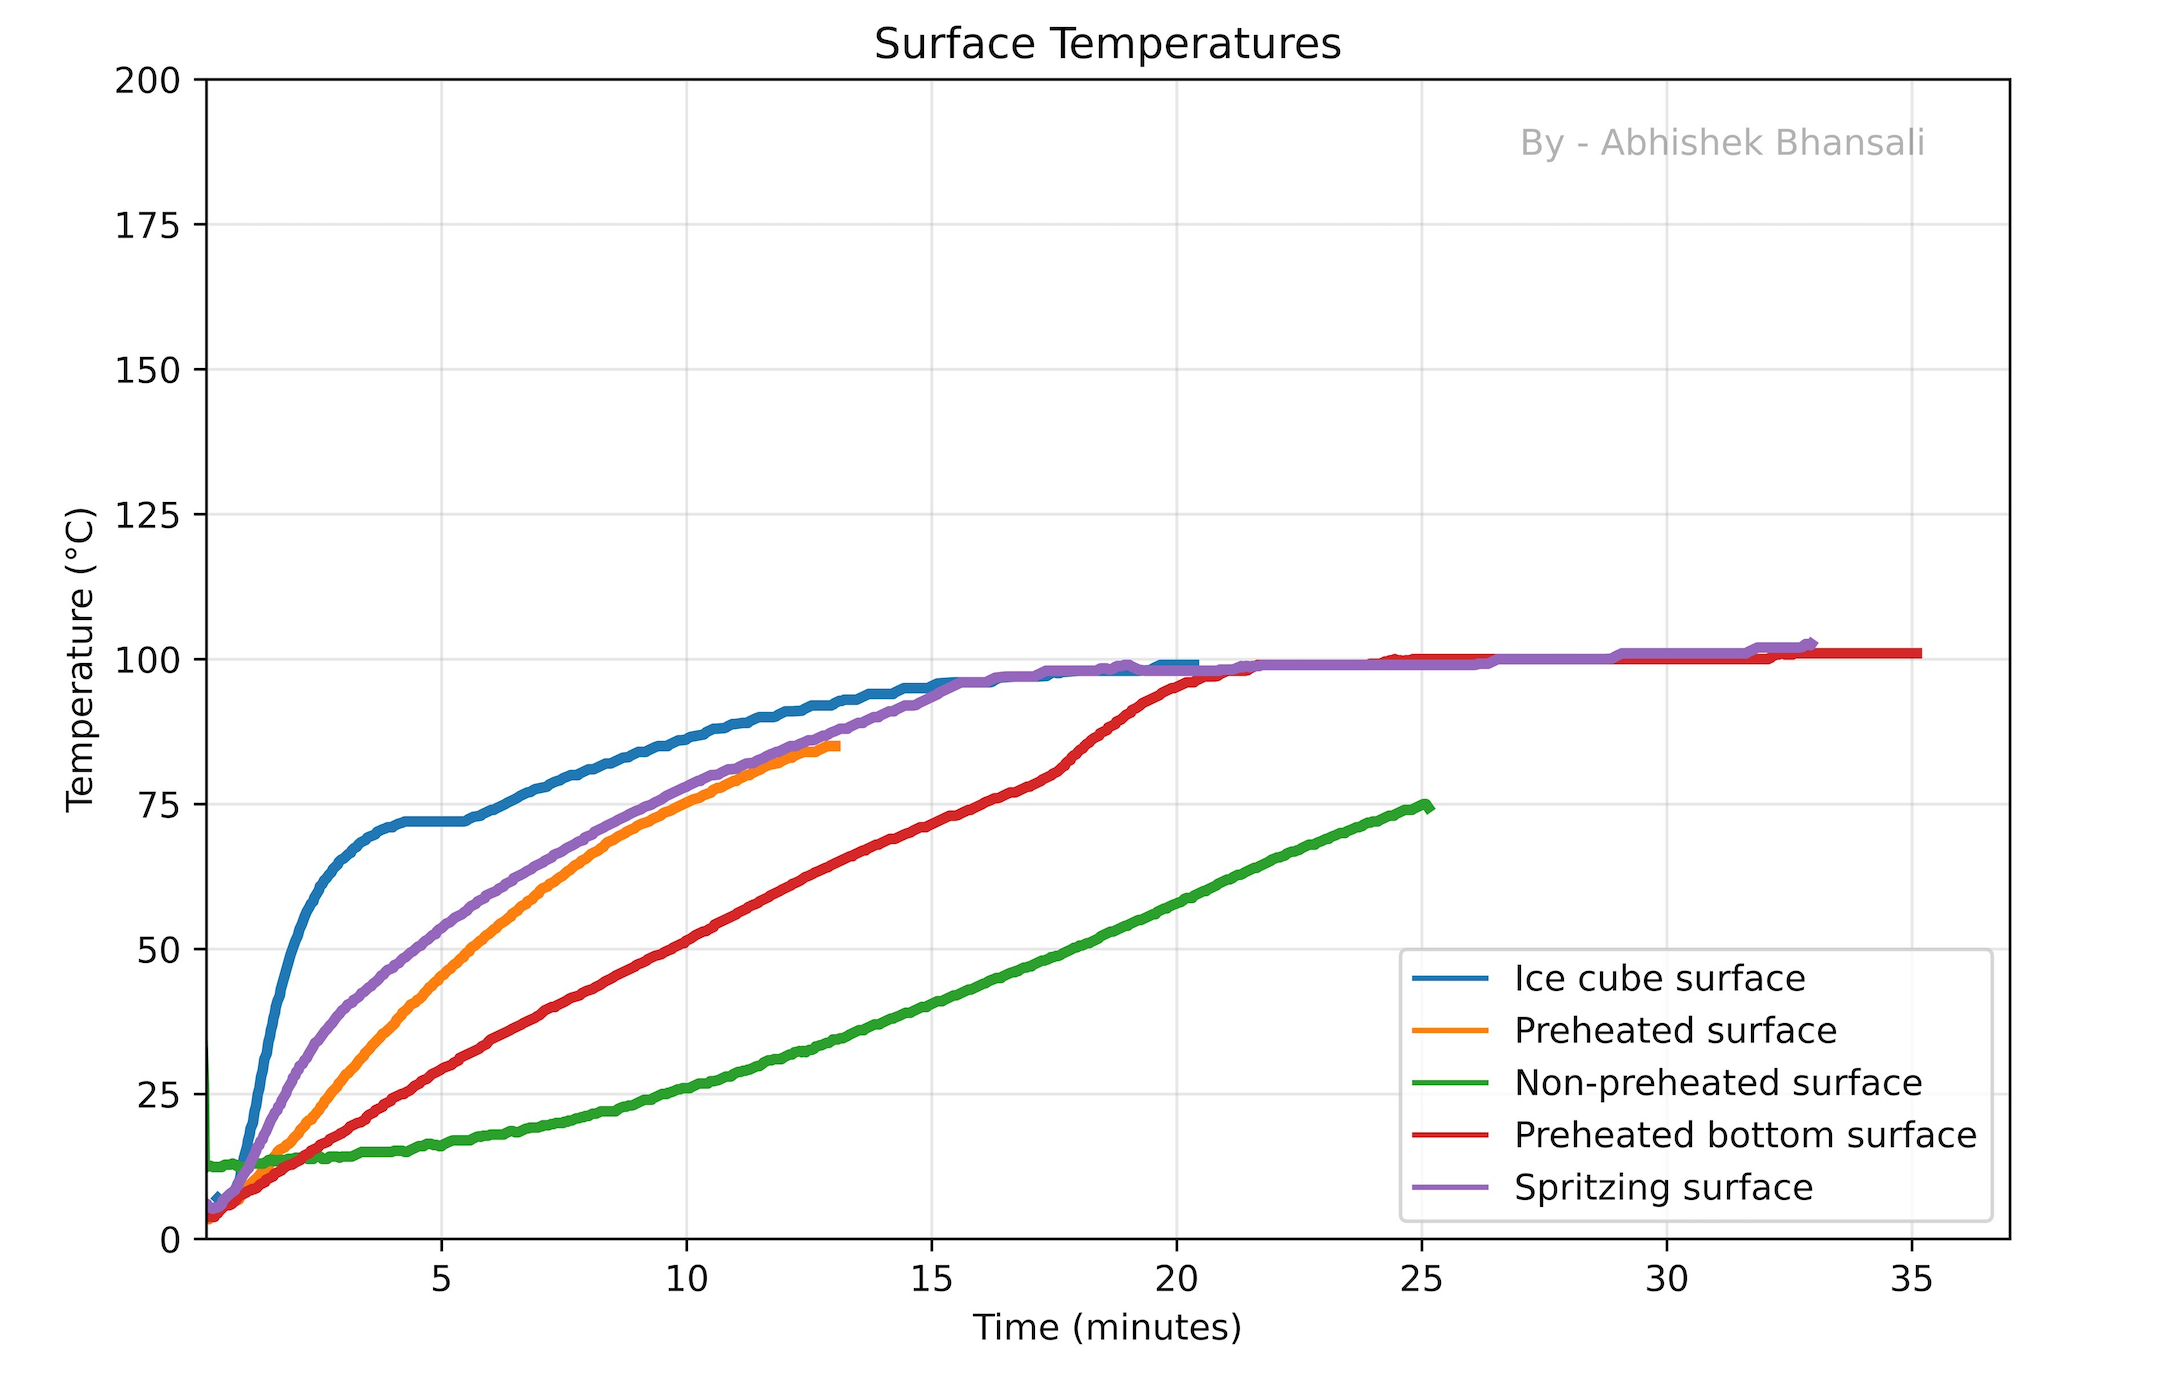
\includegraphics[width=\textwidth]{baking-experiment-temperatures.png}
%  \caption[Surface temperature for different steaming methods]{png file}
%\end{figure}

\begin{figure}[!htb]
  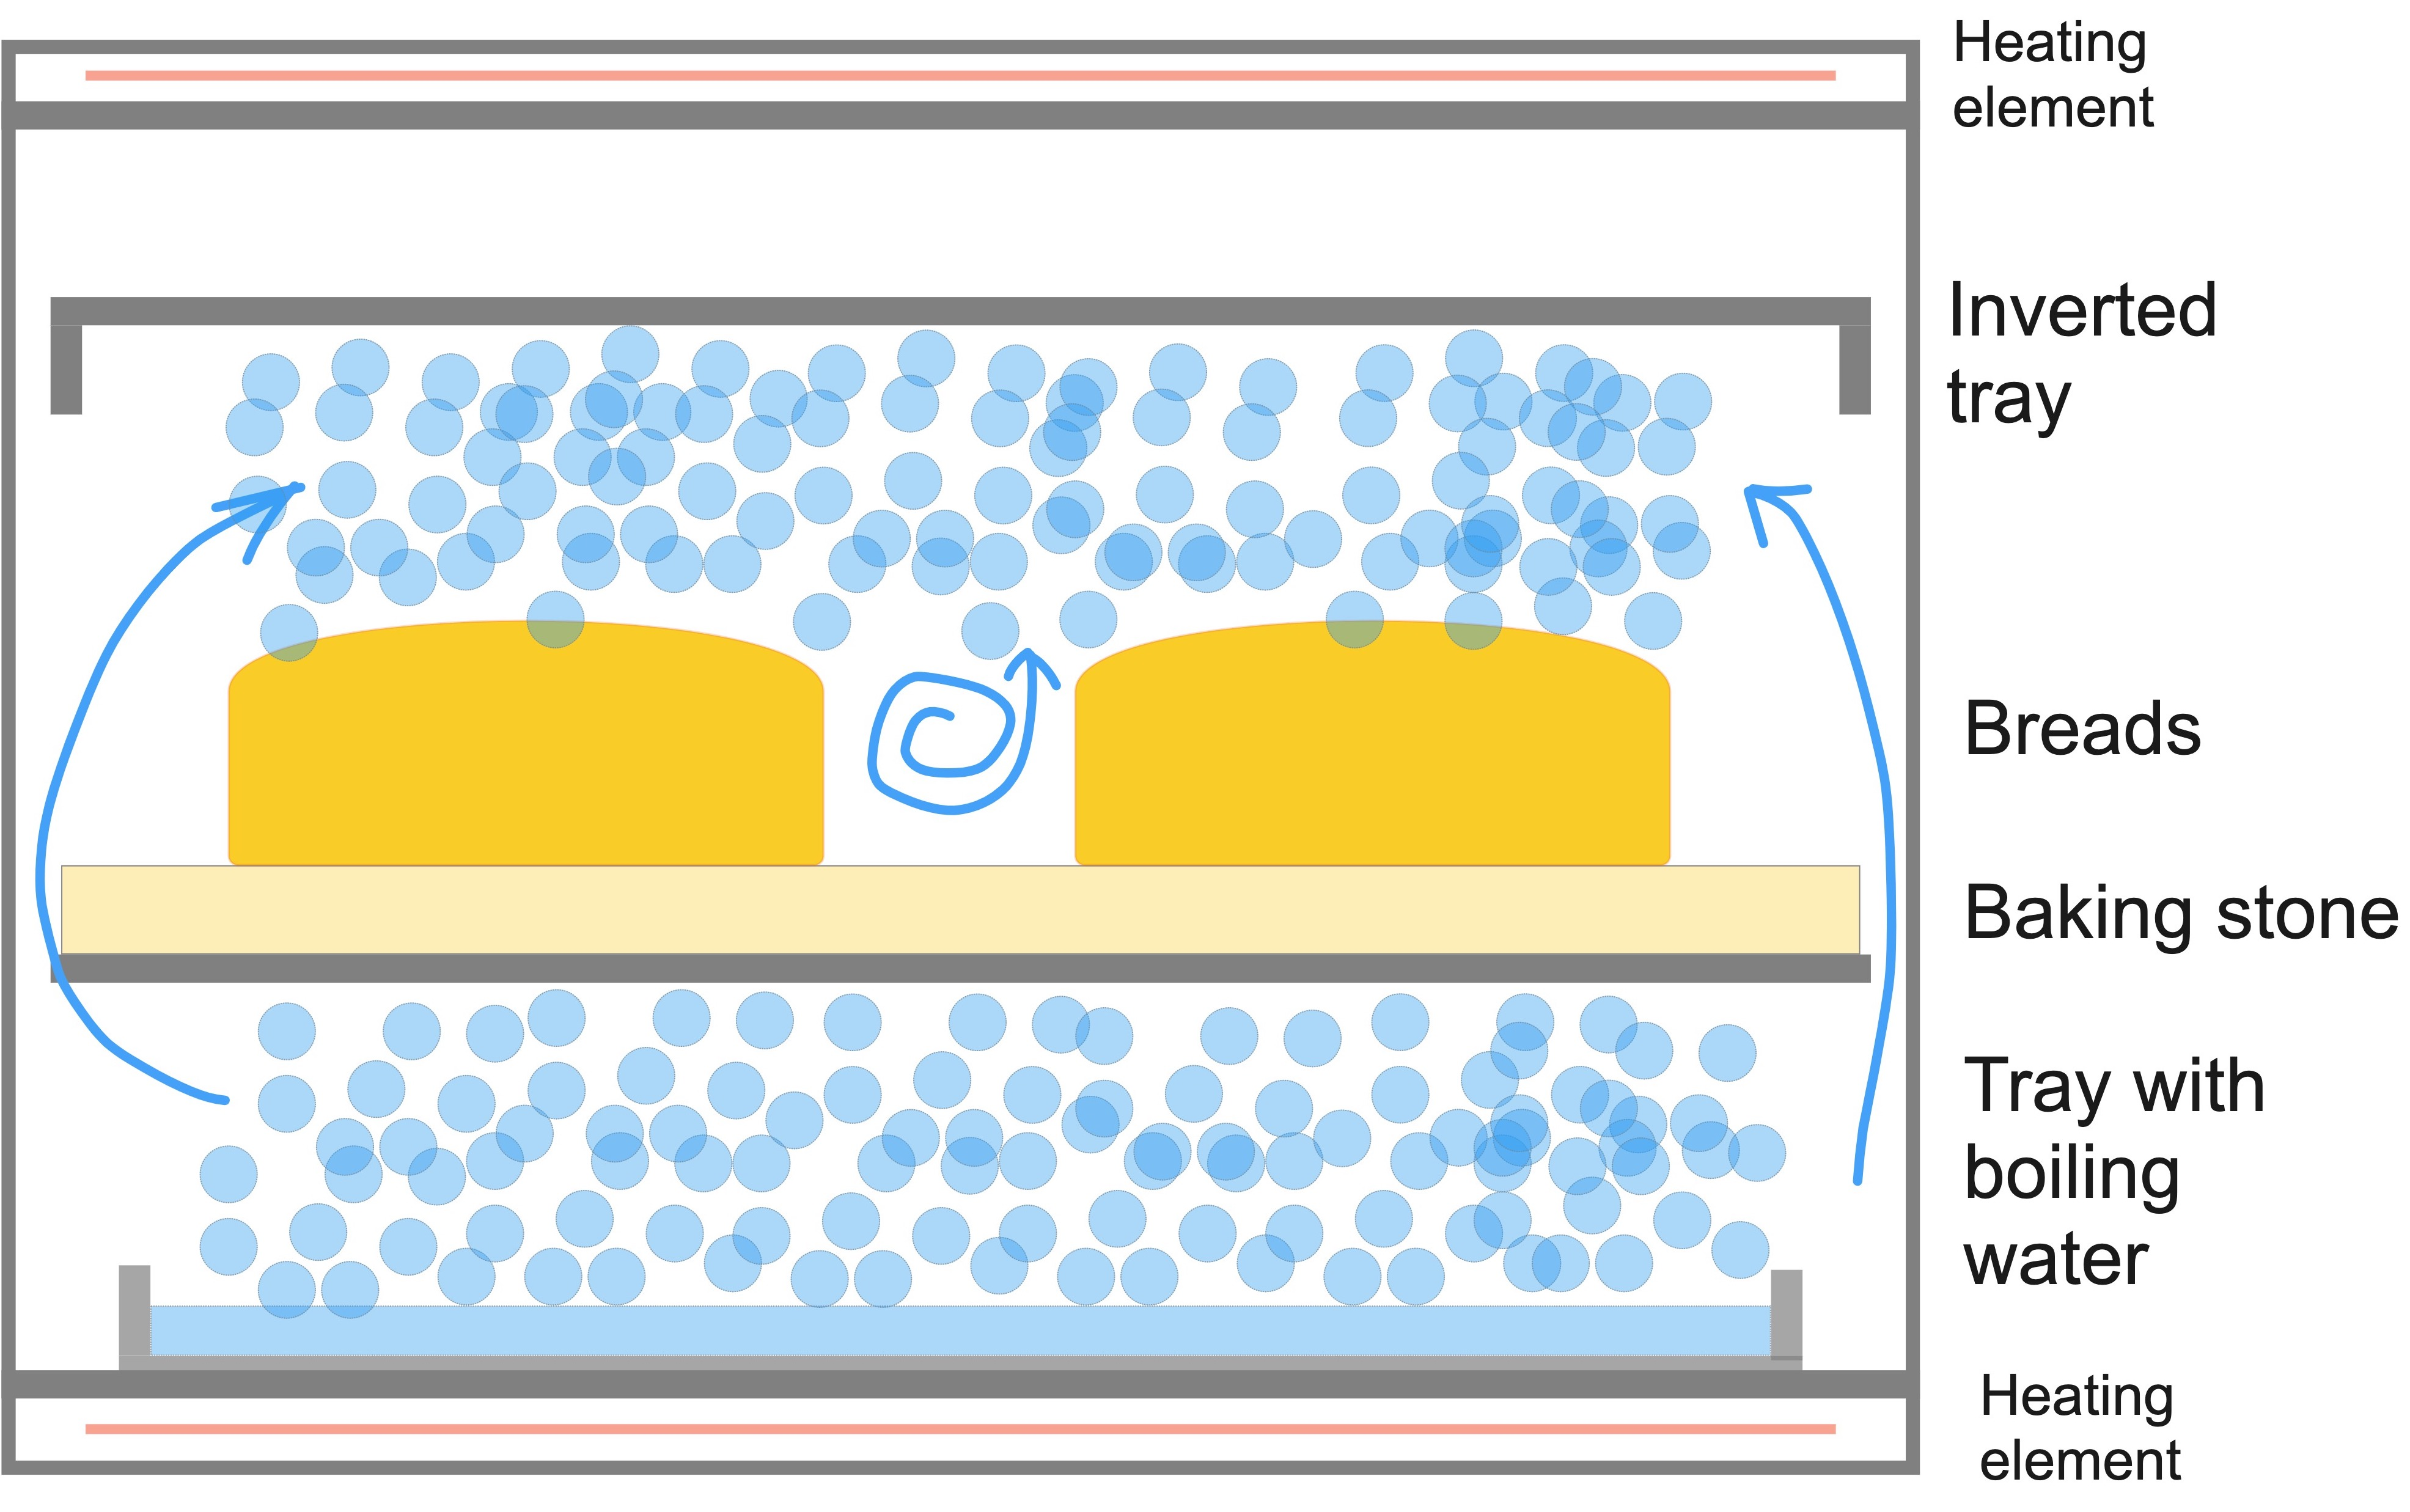
\includegraphics[width=\textwidth]{baking-process-steam.jpg}
  \caption[Steam building with inverted tray]{jpg file}%
      \label{flc:inverted-tray}
\end{figure}
If you're a hobby brewer, you'll know that it's important to keep your beer at
certain temperatures to allow the different amylases to convert the contained
starches into sugar~\cite{beer+amylase}.
This test, called the \emph{Iodine Starch Test}, involves mixing iodine into
a sample of your brew and checking the color.

% https://github.com/hendricius/the-sourdough-framework/issues/358
\begin{table}[!htb]
    \begin{center}
        \documentclass[tikz]{standalone}
\usepackage{tikz}
\usepackage{siunitx}
\DeclareSIUnit\degF{\text{°}F}

\begin{document}
\begin{tabular}{|l|l|l|l|}
\hline
\textbf{\begin{tabular}[c]{@{}l@{}}Temperature\\ in °C\end{tabular}} & \textbf{\begin{tabular}[c]{@{}l@{}}Temperature\\ in °F\end{tabular}} & \textbf{\begin{tabular}[c]{@{}l@{}}Starter\\ recently fed?\end{tabular}} & \textbf{\begin{tabular}[c]{@{}l@{}}Amount\\ of starter in\%\end{tabular}} \\ \hline
30                                                                   & 86                                                                   & Yes                                                                      & 5                                                                         \\ \hline
25                                                                   & 77                                                                   & Yes                                                                      & 10                                                                        \\ \hline
20                                                                   & 68                                                                   & Yes                                                                      & 15                                                                        \\ \hline
30                                                                   & 86                                                                   & No                                                                       & 2.5                                                                       \\ \hline
25                                                                   & 77                                                                   & No                                                                       & 5                                                                         \\ \hline
20                                                                   & 68                                                                   & No                                                                       & 10                                                                        \\ \hline
\end{tabular}
\end{document}

        \caption[Different oven types]{An overview of different oven types and
        eheir different baking methods.}
    \end{center}
\end{table}

\begin{table}[!htb]
    \begin{center}
        % TODO: Not great Looking... 
\begin{tabular}{@{}p{0.25\textwidth}ccc@{}}
\toprule
\thead{Oven type}  & \thead{Plain (no tools)} & \thead{Inverted tray} & \thead{Dutch oven} \\ \midrule
Gas                & No                       & No                    & Yes                 \\ \midrule
Convection (Fan always on) & No               & No                    & Yes                 \\ \midrule
Convection (Fan can be disabled) & No         & Yes                   & Yes                 \\ \midrule
Steam              & Yes                      & Yes                   & Yes                 \\
\bottomrule
\end{tabular}

        \caption[Different oven types]{An overview of different oven types and their
            different baking methods.}
    \end{center}
\end{table}

\end{document}
